\documentclass[pdf]{beamer}
%\mode<presentation>{}

\usepackage{amssymb,amsmath,amsthm,enumerate}
\usepackage[utf8]{inputenc}
\usepackage{array}
\usepackage[parfill]{parskip}
\usepackage{graphicx}
\usepackage{caption}
\captionsetup[figure]{labelformat=empty}
\usepackage{subcaption}
\usepackage{bm}
\usepackage{amsfonts,amscd}
%\usepackage{gensymb}
\usepackage[]{units}
\usepackage{listings}
\usepackage{multicol}
\usepackage{tcolorbox}
\usepackage{physics}
\usepackage{multimedia} % movies!
\usepackage[export]{adjustbox} % crop graphics

\usepackage{pgfpages}
\usepackage{ifthen} % package required
\usepackage[subpreambles=true]{standalone}
\usepackage{appendixnumberbeamer}
\usepackage{rotating}

\setbeameroption{show notes on second screen}

%new commands
\newcommand{\der}[2]{\frac{d#1}{d#2}}
\newcommand{\nder}[3]{\frac{d^#1 #2}{d #3 ^ #1}}
\newcommand{\pder}[2]{\frac{\partial #1}{\partial #2}}
\newcommand{\npder}[3]{\frac{\partial ^#1 #2}{\partial #3^#1}}
\newcommand{\sentencelist}{def}
\newcommand{\overbar}[1]{\mkern 1.5mu\overline{\mkern-1.5mu#1\mkern-1.5mu}\mkern 1.5mu}
\newcommand{\lined}{\overbar}
\newcommand{\perm}[2]{{}^{#1}\!P_{#2}}
\newcommand{\comb}[2]{{}^{#1}C_{#2}}
\newcommand{\intall}{\int_{-\infty}^{\infty}}
\newcommand{\Var}[1]{\text{Var}\left(#1\right)}
\newcommand{\E}[1]{\text{E}\left(#1\right)}
\newcommand{\define}{\equiv}
\newcommand{\diff}[1]{\mathrm{d}#1}
\newcommand{\empy}[1]{{\color{darkorange}\emph{#1}}}
\newcommand{\empr}[1]{{\color{cardinalred}\emph{#1}}}


\theoremstyle{remark}
\newtheorem*{remark}{Remark}
\theoremstyle{definition}

\newcommand{\examplebox}[2]{
\begin{tcolorbox}[colframe=darkcardinal,colback=boxgray,title=#1]
#2
\end{tcolorbox}}

\newcommand{\eld}[1]{\frac{d}{dt}(\frac{\partial L}{\partial \dot #1}) - \frac{\partial L}{\partial #1}=0}
\newcommand{\euler}[1]{\frac{\partial L}{\partial #1}-\frac{d}{dt}(\frac{\partial L}{\partial \dot #1})}
\newcommand{\eulerg}[1]{\frac{\partial g}{\partial #1}-\frac{d}{dt}(\frac{\partial g}{\partial \dot #1})}
\newcommand{\divg}[1]{\nabla\cdot #1}
\newcommand{\prob}[1]{P(#1\vert I)}
\DeclareMathOperator*{\argmax}{argmax}

\beamertemplatenavigationsymbolsempty

\addtobeamertemplate{footnote}{\hskip -1.8em}{}

% ================================ %
%      Section dividers            %
\newboolean{sectiontoc}
\setboolean{sectiontoc}{true} % default to true
\AtBeginSection[]
{
  \ifthenelse{\boolean{sectiontoc}}{
    \begin{frame}<beamer>{Gliederung}
      \tableofcontents[currentsection]
    \end{frame}
  }
}

\newcommand{\sectionNoDivider}[1]{
  \setboolean{sectiontoc}{false}
  \section{#1}
  \setboolean{sectiontoc}{true}
}

% \newcommand<>{\makered}[1]{{\color#2{red}#1}}
% \renewcommand<>{\hyperlink}[2]{\only#3{\beameroriginal{\hyperlink}{#1}{#2}}}
\newcommand<>{\nakedfootnote}[1]{%
  \begingroup
  \renewcommand<>\thefootnote{}\footnote#2{#1}%
  \addtocounter{footnote}{-1}%
  \endgroup
}

\AtBeginSection[]
{
	\ifthenelse{\boolean{sectiontoc}}{
	  \begin{frame}<beamer>
	    \frametitle{\insertsectionhead}
	    \tableofcontents[currentsection,hideallsubsections]
	  \end{frame}
	}
}

\AtBeginSubsection[]
{
  \begin{frame}<beamer>
    \frametitle{Outline for \insertsectionhead}
    \tableofcontents[
        currentsection,
        currentsubsection,
        subsectionstyle=show/shaded/hide
    ]
  \end{frame}
}

\usetheme{Stanford}
\def \i  {\item}
\def \ai {\item[] \quad \arrowbullet}
\newcommand \si[1]{\item[] \quad \bulletcolor{#1}}
\def \wi {\item[] \quad $\ \phantom{\Rightarrow}\ $}
\def \bi {\begin{itemize}\item}
\def \ei {\end{itemize}}
\def \be {\begin{equation*}}
\def \ee {\end{equation*}}
\def \bie {$\displaystyle{}
\def \eie {{\ }$}}
\def \bsie {\small$\displaystyle{}
\def \esie {{\ }$}\normalsize\selectfont}
\def \bse {\small\begin{equation*}}
\def \ese {\end{equation*}\normalsize}
\def \bfe {\footnotesize\begin{equation*}}
\def \efe {\end{equation*}\normalsize}
\renewcommand \le[1] {\\ \medskip \lefteqn{\hspace{1cm}#1} \medskip}
\def \bex {\begin{example}}
\def \eex {\end{example}}
\def \bfig {\begin{figure}}
\def \efig {\end{figure}}
\def \btheo {\begin{theorem}}
\def \etheo {\end{theorem}}
\def \bc {\begin{columns}}
\def \ec {\end{columns}}
\def \btab {\begin{tabbing}}
\def \etab {\end{tabbing}\svneg\svneg}
\newcommand \col[1]{\column{#1\linewidth}}
\def\vneg  {\vspace{-5mm}}
\def\lvneg {\vspace{-10mm}}
\def\svneg {\vspace{-2mm}}
\def\tvneg {\vspace{-1mm}}
\def\vpos  {\vspace{5mm}}
\def\lvpos {\vspace{10mm}}
\def\svpos {\vspace{2mm}}
\def\tvpos {\vspace{1mm}}
\def\hneg  {\hspace{-5mm}}
\def\lhneg {\hspace{-10mm}}
\def\shneg {\hspace{-2mm}}
\def\thneg {\hspace{-1mm}}
\def\hpos  {\hspace{5mm}}
\def\lhpos {\hspace{10mm}}
\def\shpos {\hspace{2mm}}

\logo{
\includegraphics[height=0.5in]{./style_files_stanford/SU_New_BlockStree_2color.png}}



\title[\insertsectionhead]{Variational Bayesian Methods (in Neuroscience)}
% \title[PhD Qualifying Exam]{Causal models of brain dynamics}

\begin{document}



\author[Tyler Benster \& Aaron Andalman, CNJC]{
	\begin{tabular}{c}
	\Large
	Tyler Benster \& Aaron Andalman\\
    \footnotesize
    Deisseroth (Tyler \& Aaron) and Druckmann (Tyler) Labs
\end{tabular}
\vspace{-2ex}
}

\institute{
	\vspace{2ex}
	
\includegraphics[height=0.4in]{./style_files_stanford/SU_New_BlockStree_2color.png}\\
	Computational Neuroscience Journal Club\\
	Stanford University}

\date{July 10, 2019}

\begin{noheadline}
\begin{frame}\maketitle\end{frame}
\end{noheadline}

%%%%%%%%%%%%%%%%%%%% Actual start %%%%%%%%%%%%%%%%%%%%%%%%%%%%%

\begin{frame}<beamer>
    \frametitle{Roadmap}
    \tableofcontents[subsectionstyle=hide]\
\end{frame}

\newcommand{\Zero}{Introduction: Why care about the distribution of data?}
\newcommand{\One}{Problem: Analyzing high dimensional data is hard}
\newcommand{\Two}{Solution: Variational Methods}
\newcommand{\Three}{Example: variational autoencoder}

\section{\Zero}

\begin{frame}[t]{The probability distribution revolution}
	\begin{multicols}{2}
		\begin{itemize}
			\item Karl Pearson (1857-1936) came with the idea that scientific measurements should be conceived as coming from probability distributions.
			\item Scientific measurements are just random reflections of the underlying truth that is the distribution.
			\item “A great book on the
history of statistics” $\rightarrow$ Aaron
			\item
		\end{itemize}

		\columnbreak

		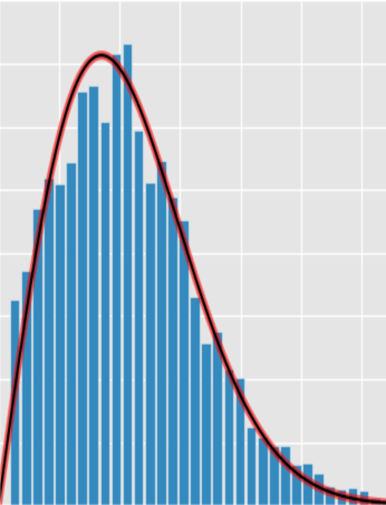
\includegraphics[width=0.25\textwidth]{media/distribution}
		\linebreak
		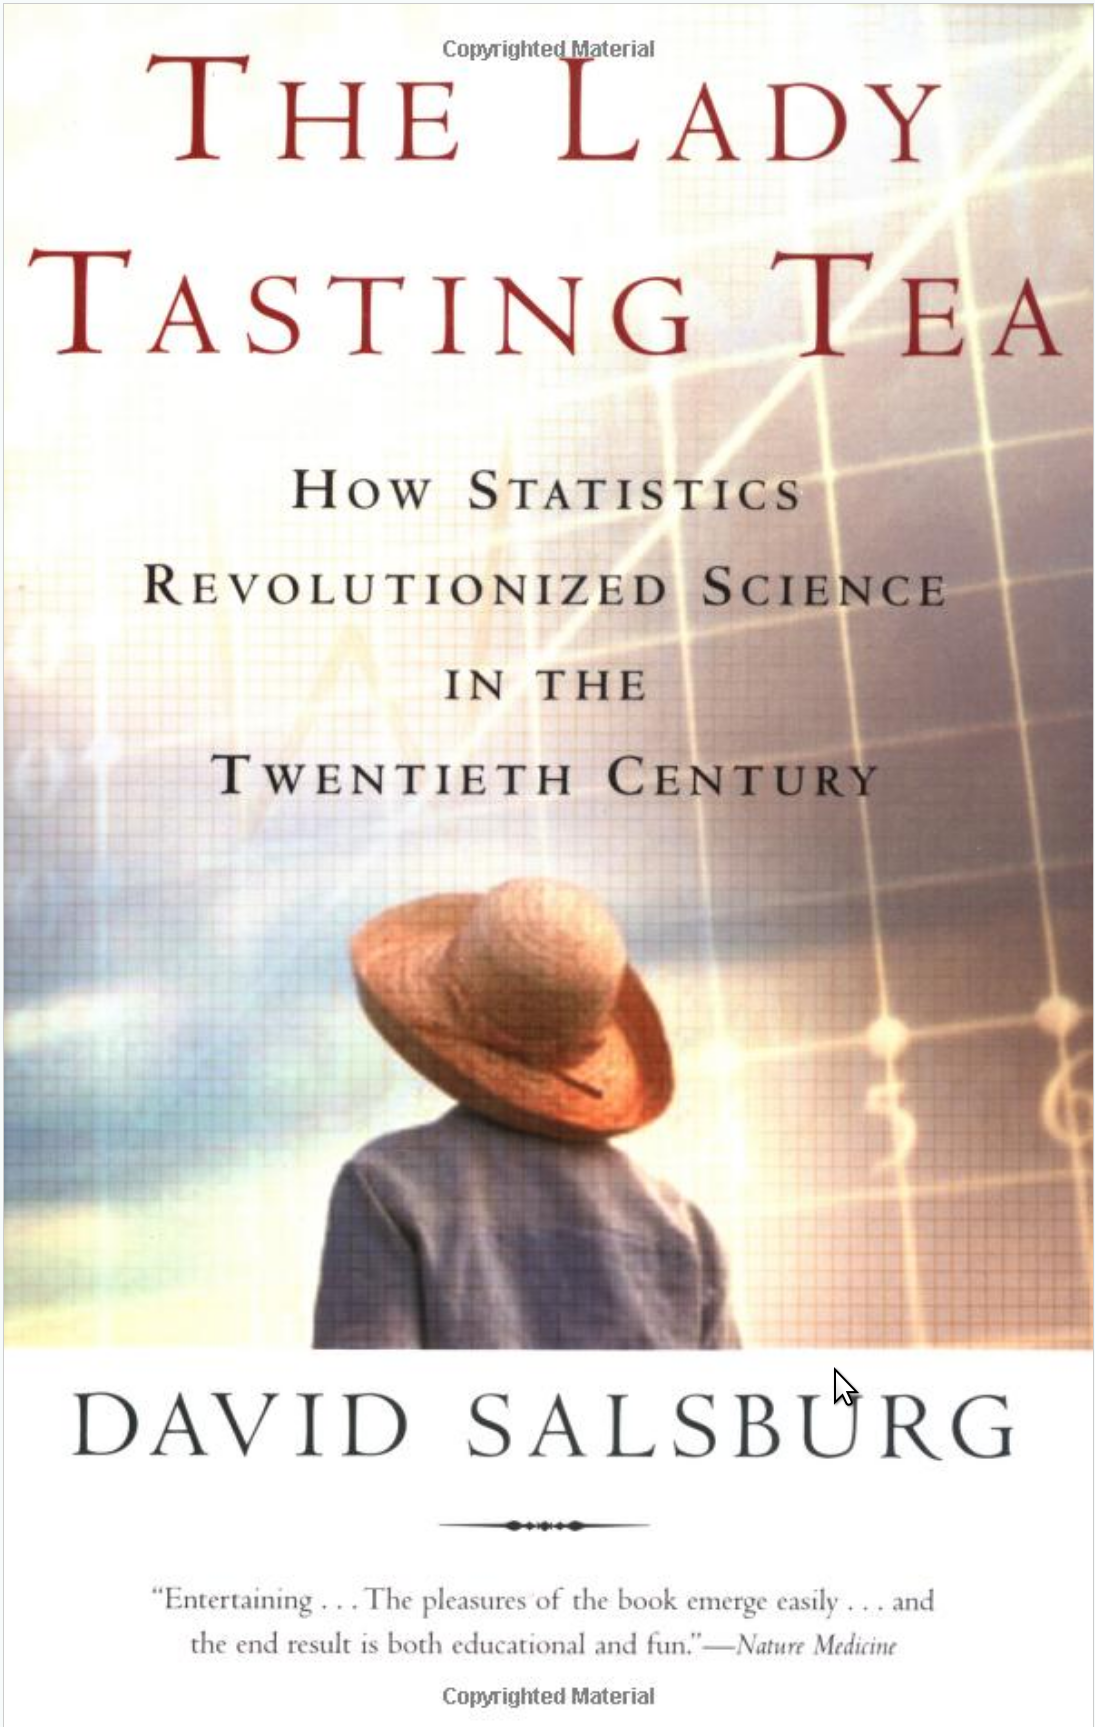
\includegraphics[width=0.25\textwidth]{media/book}
	\end{multicols}
\end{frame}

\begin{frame}[t]{The power of probability distributions}
	Distributions allow scientists to:
	\begin{itemize}
		\item Understand scientific measurement
		\item Predict the probability of specific data
		\item Test specific hypothesis (p-values)
		\item Produce generative models
		\item Better conceptual understanding data.
	\end{itemize}
\end{frame}
%--- Next Frame ---%

\begin{frame}[t]{Estimating distributions from data}
	\begin{multicols}{2}
		Low-Dimensional:
		\begin{itemize}
			\item Great tools to fit and understand the underlying probability distribution of data.
		\end{itemize}
		\vfill\columnbreak
		High-Dimensional:
		\begin{itemize}
			\item In some cases, classical statistical tools are insufficient.
			\item Problematic for modern neuroscience:
			\item Thousands of electrodes.
			\item Millions of voxels.
		\end{itemize}
	\end{multicols}
\end{frame}
%--- Next Frame ---%

\begin{frame}[t]{Variational Bayesian Methods}
	Estimate the probability distribution of high-dimensional neural data.
	\begin{itemize}
		\item Compute the probability of observing a particular neural state.
		\item Sample neural states/trajectory from the estimate.
		\item Generate statistics / test hypotheses
		\item Estimate latent factors/states that drive the observations.
		\item Reduce dimensionality (with advantages over other methods, e.g. PCA, T-SNE)
	\end{itemize}
\end{frame}
%--- Next Frame ---%

\section{\One}

\begin{frame}[t]{Approximating the area of a circle with Monte Carlo}
	\begin{center}
		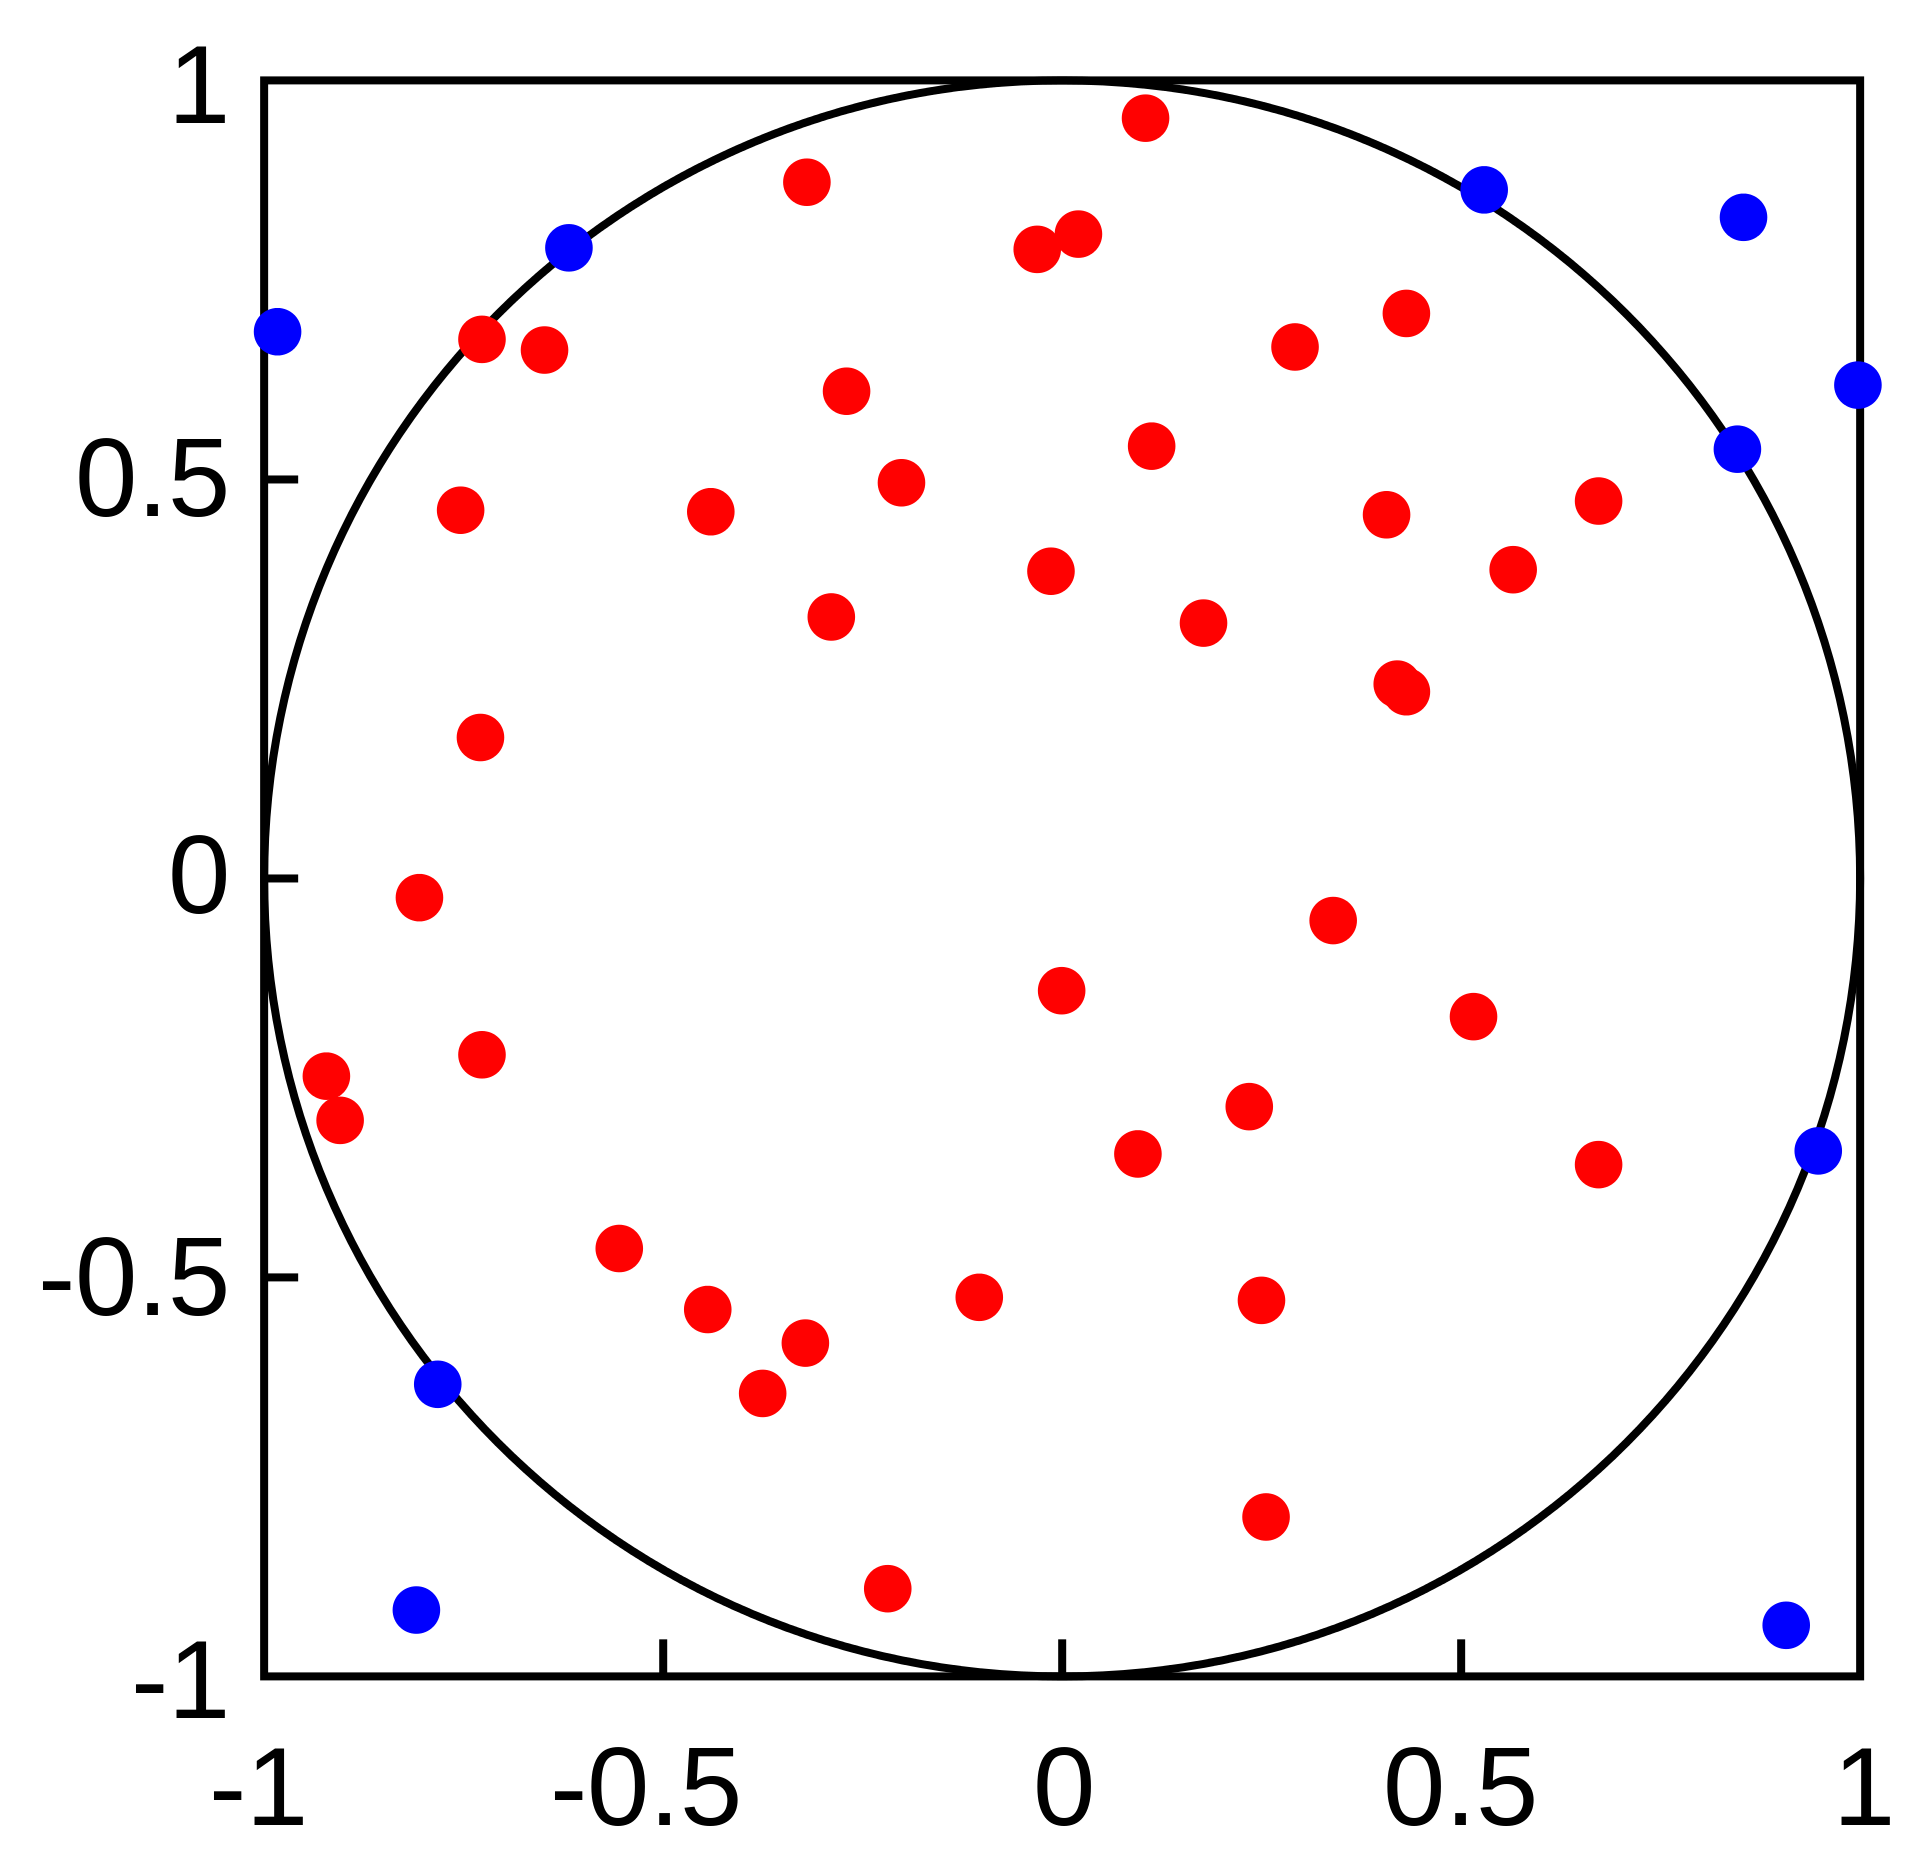
\includegraphics[height=0.75\textheight]{media/2d_monte_carlo}
		\linebreak
		40/50 samples in circle gives area of $4 * 0.8 = 3.2 \approx \pi$. $\sim 2\%$ error
	\end{center}
	\nakedfootnote{CCO 1.0, wikimedia, MonteCarloIntegrationCircle.svg}
\end{frame}

\begin{frame}[t]{Useful for analytically intractable integrals}
	\begin{center}
		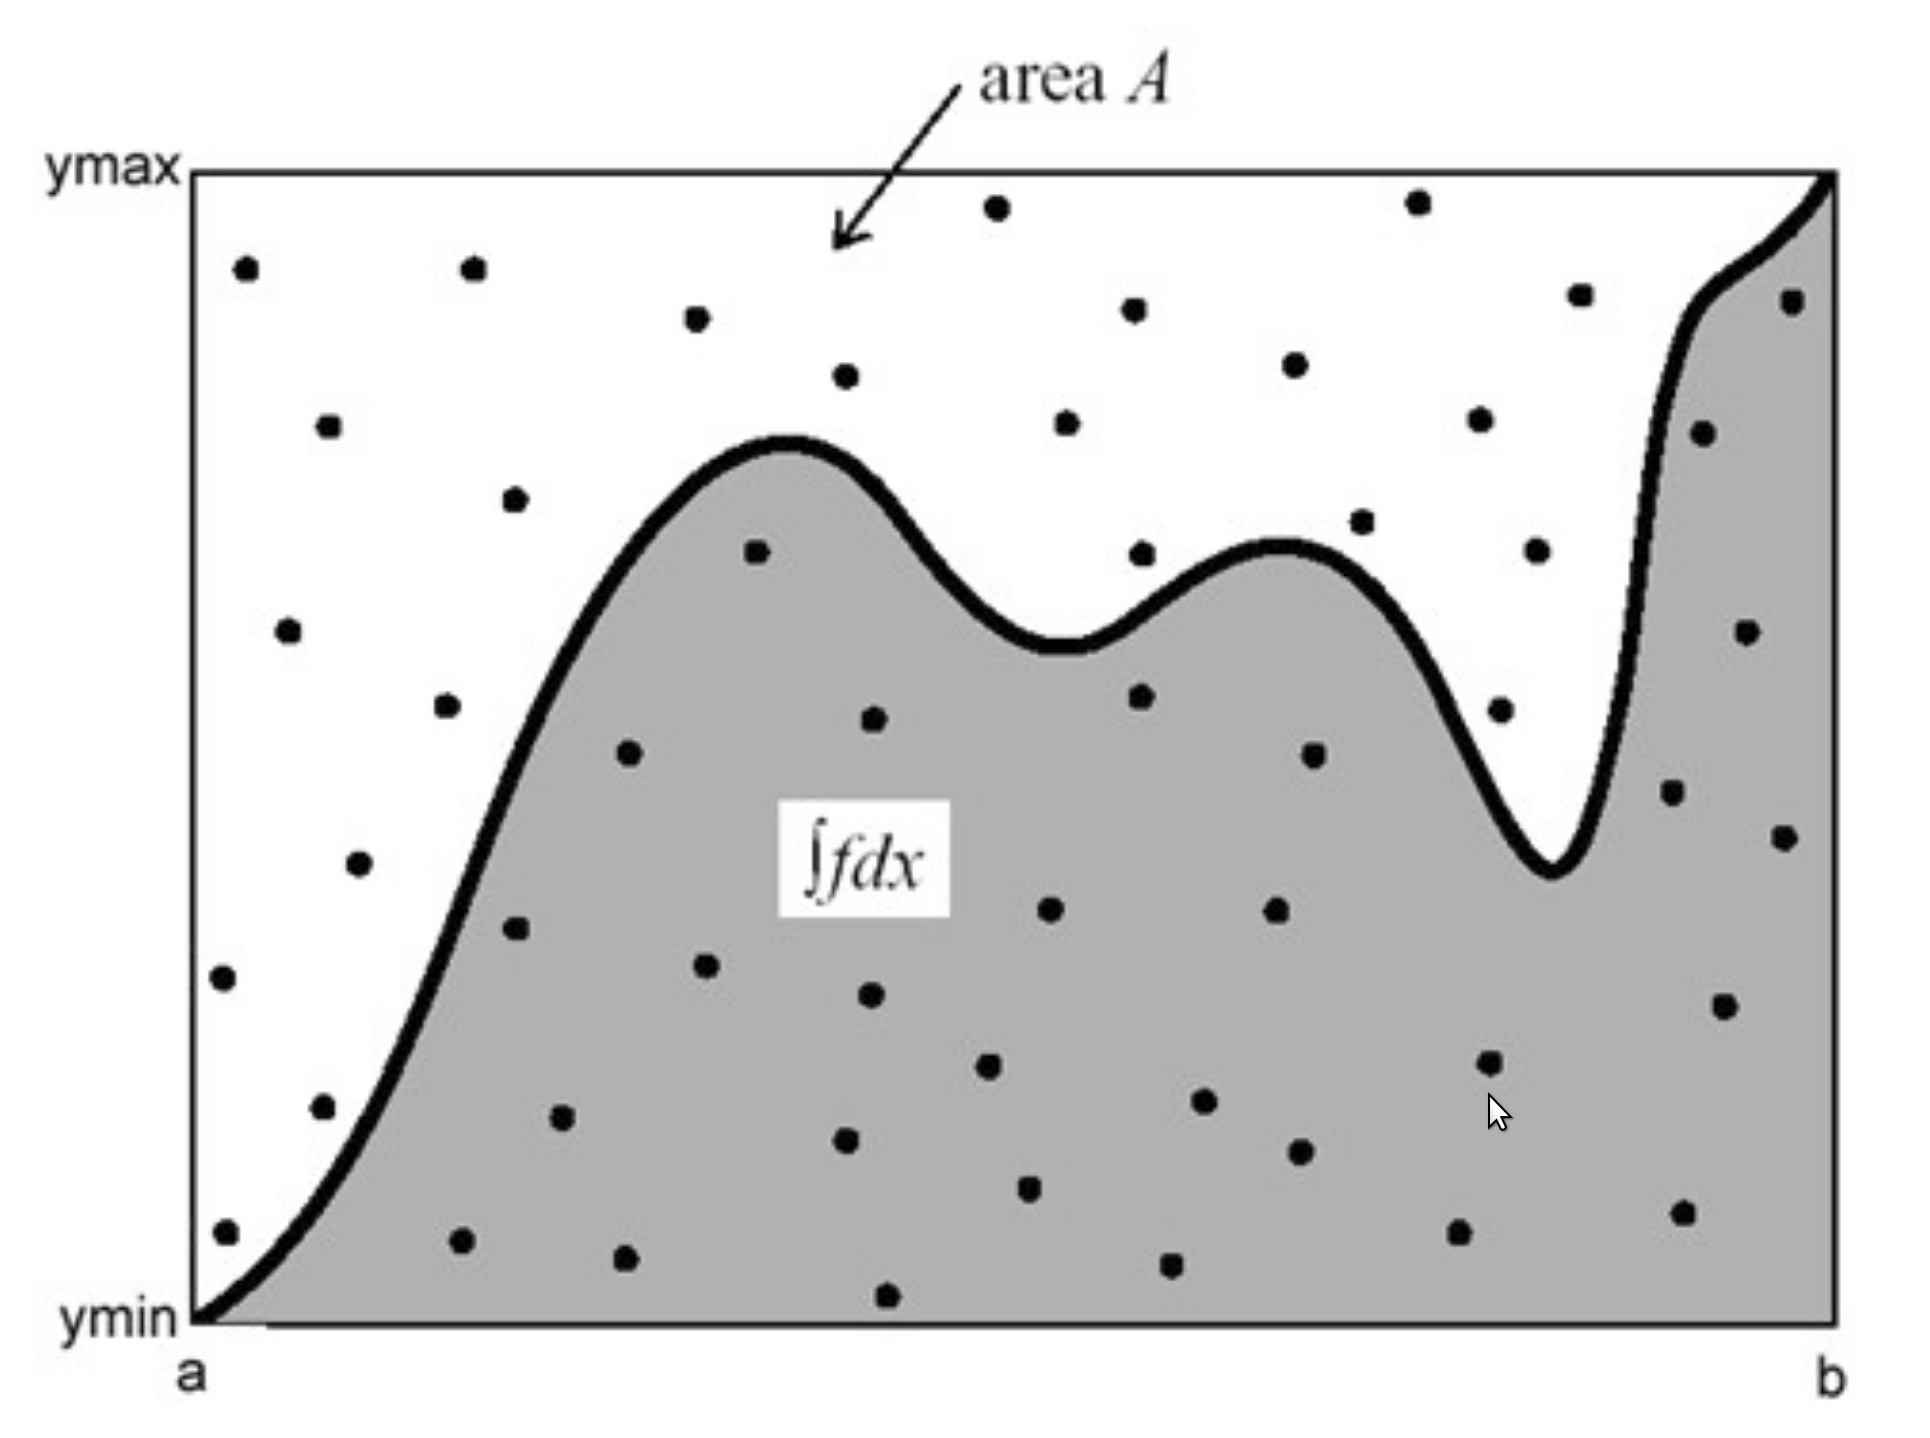
\includegraphics[height=0.75\textheight]{media/mc_integration}
	\end{center}
	\nakedfootnote{Robert Lin - Monte Carlo Integration }
\end{frame}

\begin{frame}[t]{Extension to unit hypercube}
	We can approximate a high-dimensional integral using a Monte Carlo approximation:
	\begin{align*}
		\int_0^1 \cdots \int_0^1 g(x_1,\dots,x_n) dx_1,\dots,dx_n
			\approx \frac{1}{N}\sum_{j=1}^N g(\bar{x}_j)
	\end{align*}
	where $\bar{x}_1,\dots,\bar{x}_N \sim \mathcal{U}(0,1)$ is the i\textsuperscript{th} random sample
\end{frame}


\begin{frame}[t]{Performance scales poorly with number of
	dimensions}
	\center
	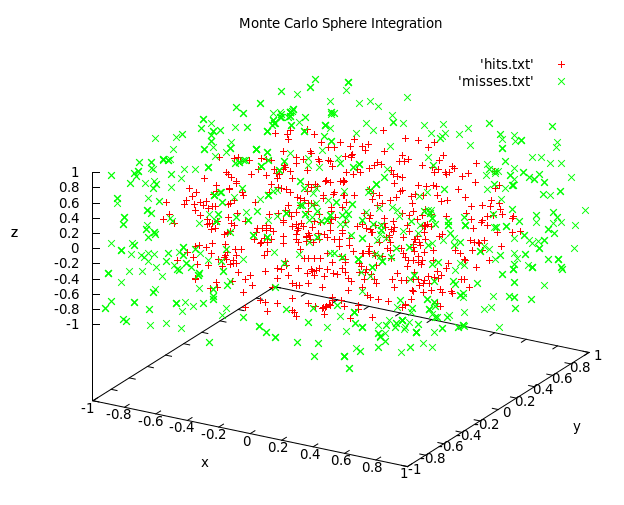
\includegraphics[height=0.8\textheight]{media/3d_monte_carlo}
	\linebreak
	1000 samples, estimate = 4.072, actual = 4.189, $\sim 3\%$ error
	\nakedfootnote{http://www2.hawaii.edu/~yuxian/phys305/a6/}
\end{frame}

\section{\Two}

\begin{frame}[t]{Alternate approach: Variational Bayes}
	\center
	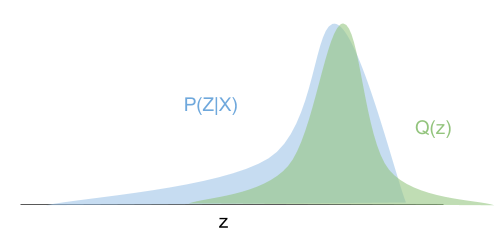
\includegraphics[width=\textwidth]{media/variational_gaussian}
\end{frame}

\section{\Three}

\begin{frame}[t]{Demo}
	\vfill
	\center
	\huge https://bit.ly/2LcEhow
	\vfill
\end{frame}

\begin{frame}[t]{Summary}
	\begin{itemize}
		\item \One \begin{itemize}
				\item
			\end{itemize}
		\item \Two \begin{itemize}
			\item
		\end{itemize}
		\item \Three \begin{itemize}
			\item
		\end{itemize}
	\end{itemize}
\end{frame}

\section{Discussion: Neuroscience applications}
\begin{frame}[t]{Example: LFADS}
	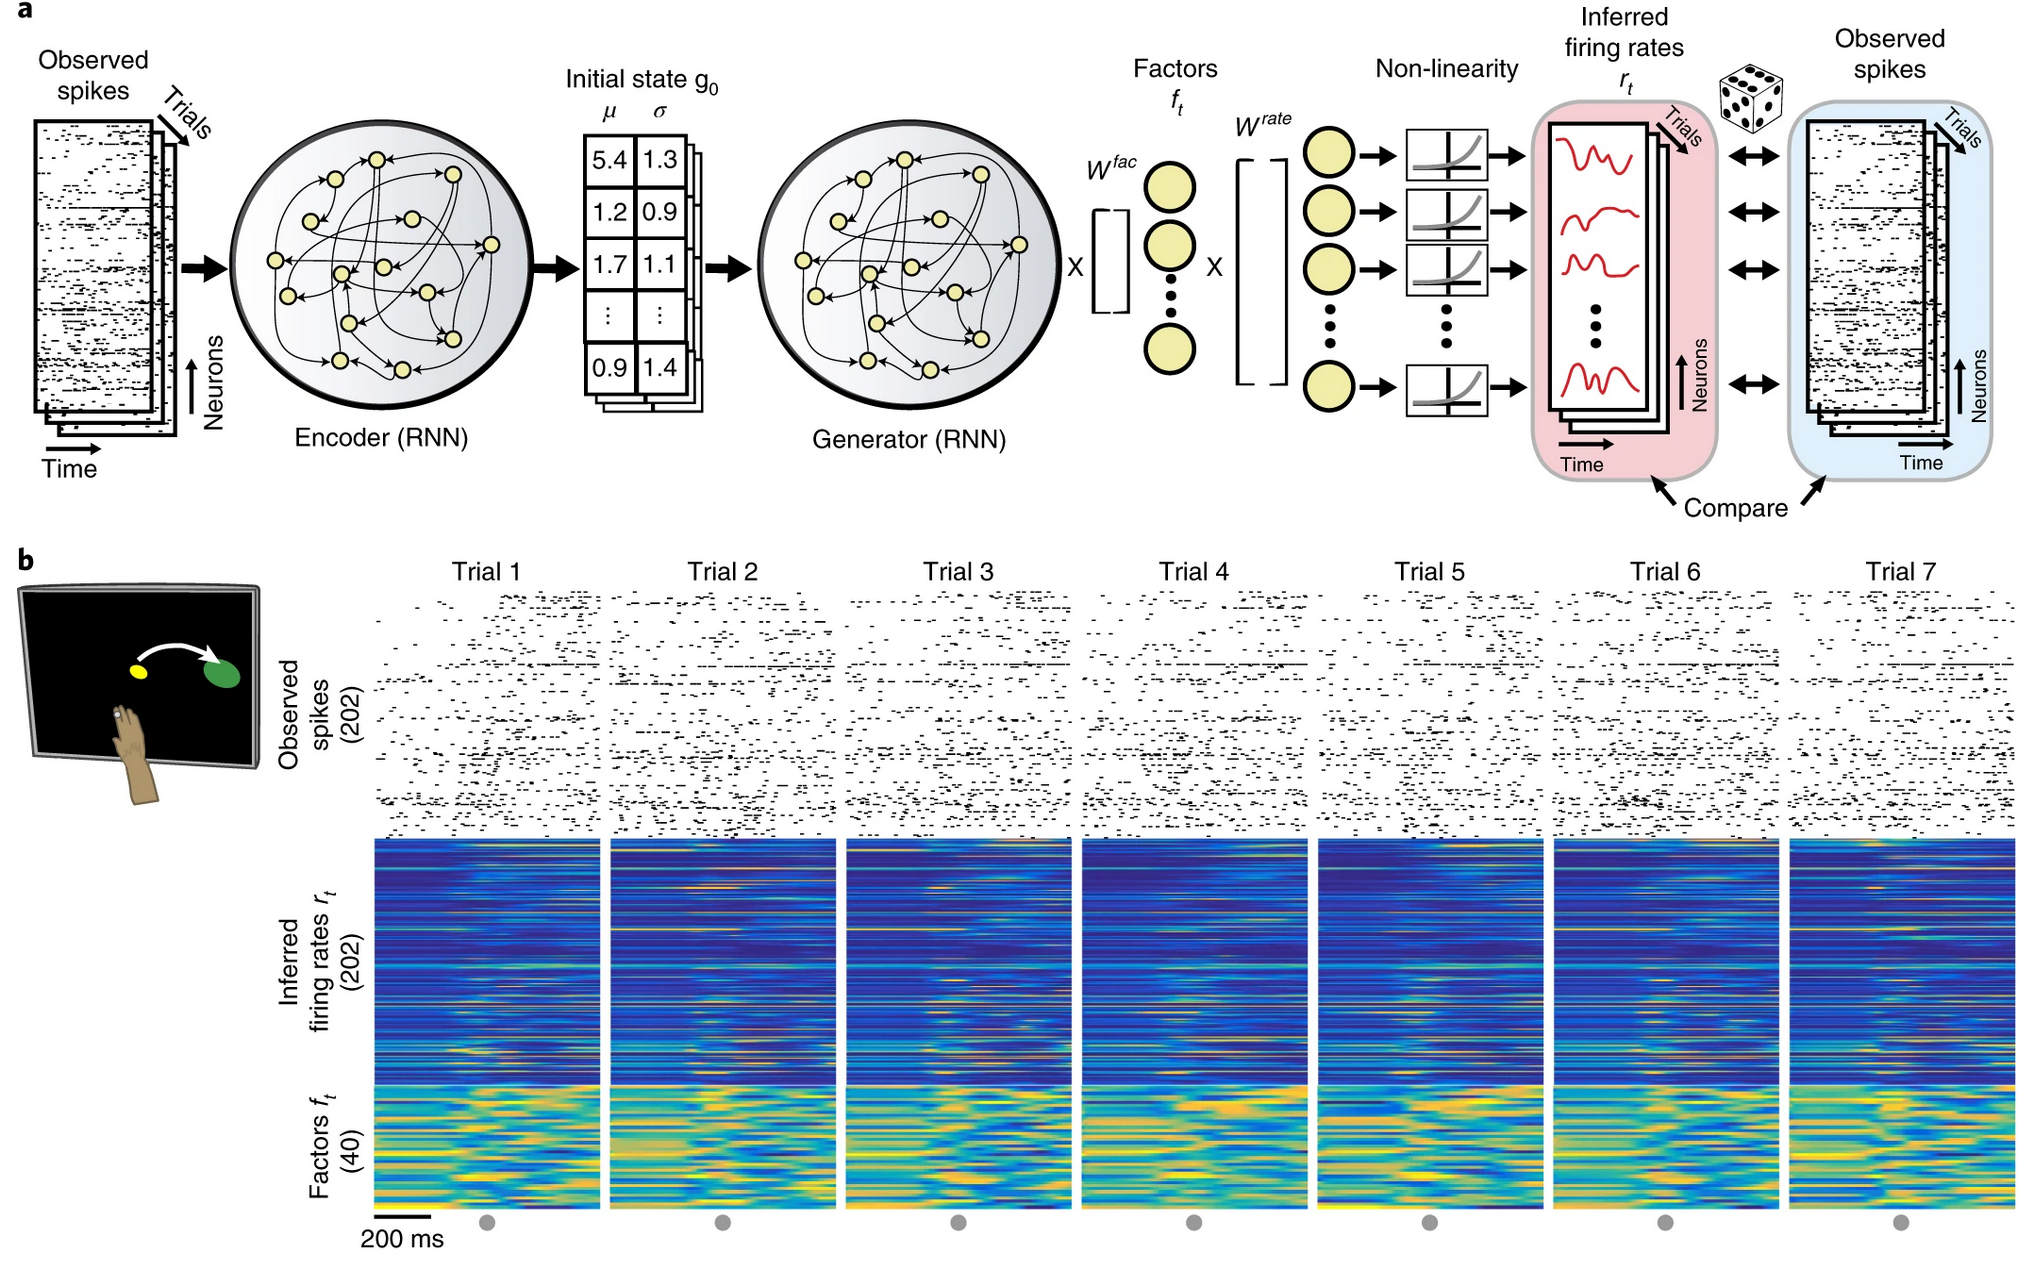
\includegraphics[width=\textwidth]{media/LFADS}
\end{frame}
%--- Next Frame ---%

\end{document}
